\documentclass{article}
\usepackage[utf8]{inputenc}
\usepackage[T1]{fontenc}
\usepackage[margin=1in]{geometry}
\usepackage{booktabs}
\usepackage{graphicx}
\usepackage[french]{babel}

\title{Rapport projet taquin}
\author{Julien Basson, Vincent Bonnecuelle, Elisa Lescarret et Jibril Saffi}
\date{\today}

\begin{document}
\maketitle
\section{Algorithme IDA\up{*}}
\begin{center}
\begin{tabular}{lllll}
    \toprule
    Fichier de test & Coups minimum & Nombre de nœuds visités & Taille maximum & Temps (en s)\\
    \midrule
    sp000.txt & 13 & 353     & 13 & 0,033\\
    sp001.txt & 15 & 7205    & 15 & 0,110\\
    sp002.txt & 25 & 5795540 & 25 & 7,440\\
    sp003.txt & 9  & 60      & 9  & 0,027\\
    sp004.txt & 21 & 683786  & 21 & 1,344\\
    sp005.txt & 21 & 378346  & 21 & 0,723\\
    sp006.txt & 22 & 1108673 & 22 & 1,768\\
    sp007.txt & 27 & 4078703 & 27 & 5,154\\
    \bottomrule
\end{tabular}
\end{center}
\begin{figure}[h]
\begin{minipage}{0.5\linewidth}
    \centering
    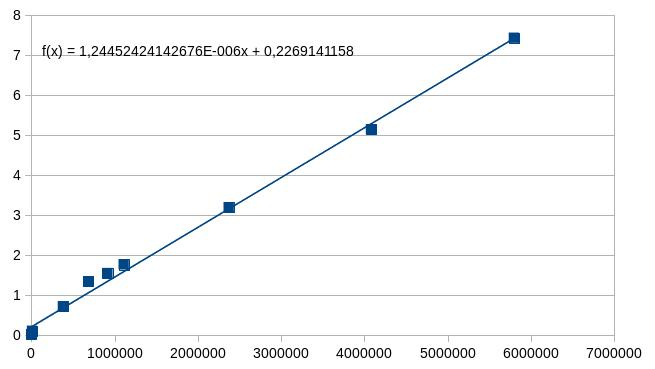
\includegraphics[width=0.8\linewidth]{time_v_nodes.png}
    \caption{Temps en fonction du nombre de noeuds visités}
\end{minipage}
\hspace{1cm}
\begin{minipage}{0.5\linewidth}
    \centering
    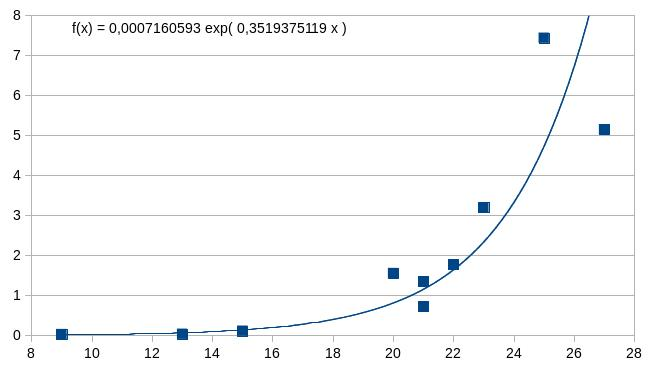
\includegraphics[width=0.8\linewidth]{time_v_solution_size.png}
    \caption{Temps en fonction de la taille de la solution optimale}
\end{minipage}
\end{figure}
Outils utilisés:
\begin{itemize}
    \item OpenJDK 1.8.0\_60
    \item OpenJFX 8.0.76\--ea
\end{itemize}
\end{document}
